%%%%%%%%%%%%%%%%%%%%%%%%%%%%%%%%%%%%%%%%%%%%%%%%%%%%%%%%%%%%%%%%%%%%%%%%%%%%%
% PACKAGES AND USUAL STUFF

\documentclass[helv,dvipsnames]{apa7}

\usepackage{xcolor} %for different type of colour. wtatch out for the package option crash message :https://nuanceabounds.org/fix-latex-package-option-clash-error-passoptionstopackage/
\usepackage{geometry}
\usepackage{ulem}%to strike out the text
\geometry{a4paper}
\usepackage[american]{babel}
\usepackage{csquotes}
\usepackage{graphicx}
\usepackage[style=apa,sortcites=true,sorting=nyt,backend=biber]{biblatex}
\DeclareLanguageMapping{american}{american-apa}
\addbibresource{bibliography.bib}
\usepackage{fancyhdr}
\usepackage{makecell}
\usepackage{amsmath}
\pagestyle{fancy} %to use fancy, you need the package fancyhdr


%%%%%%%%%%%%%%%%%%%%%%%%%%%%%%%%%%%%%%%%%%%%%%%%%%%%%%%%%%%%%%%%%%%%%%%%%%%%%%%
%HEADERS AND FOOTERS 

\rightmark
\fancyhf{} % sets both header and footer to nothing
\renewcommand{\headrulewidth}{0pt}
\fancyheadoffset[R]{-25pt}
\fancyhead[L]{Pre-study - Proposal}
\renewcommand{\headrulewidth}{0.1mm}
\renewcommand{\footrulewidth}{0.1mm}
\fancyfoot[R]{\thepage %\ of \pageref{LastMainPage}
}
\fancyfoot[L]{BenMobility - \today}

%\lhead{}
\rhead{{
	\begin{picture}(0,0)
	
\includegraphics[height=1.2cm]{Figures/EPFL_logo.eps}
\end{picture}}}
%%%%%%%%%%%%%%%%%%%%%%%%%%%%%%%%%%%%%%%%%%%%%%%%%%%%%%%%%%%%%%%%%%%%%%%%%%%%%%%%%%%%%
% DOCUMENT BEGINS

% for quote “” %
\begin{document}
\section{Preface}
Right before starting my master degree at EPFL, I was working on a feasible study about interoperability between an inter-city train and a light rail train for a Canadian rail consultant firm. The project was captivating and very complex. However, I felt that my bachelor degree in civil engineering wasn't enough to provide the necessary tools to build a specialized career in the railways. Therefore, I decided to get a master degree in transport and mobility, with in mind the expectation of learning useful skills in the field of railways.
\par While I was looking for a pre-study during my second semester at EPFL, I came across an article in a newspaper about Canton de Vaud seeking for a new railway strategy for 2050~(\cite{vaud2050} and \cite{tempsvision2050}). 
\begin{figure}[h]
    \centering
    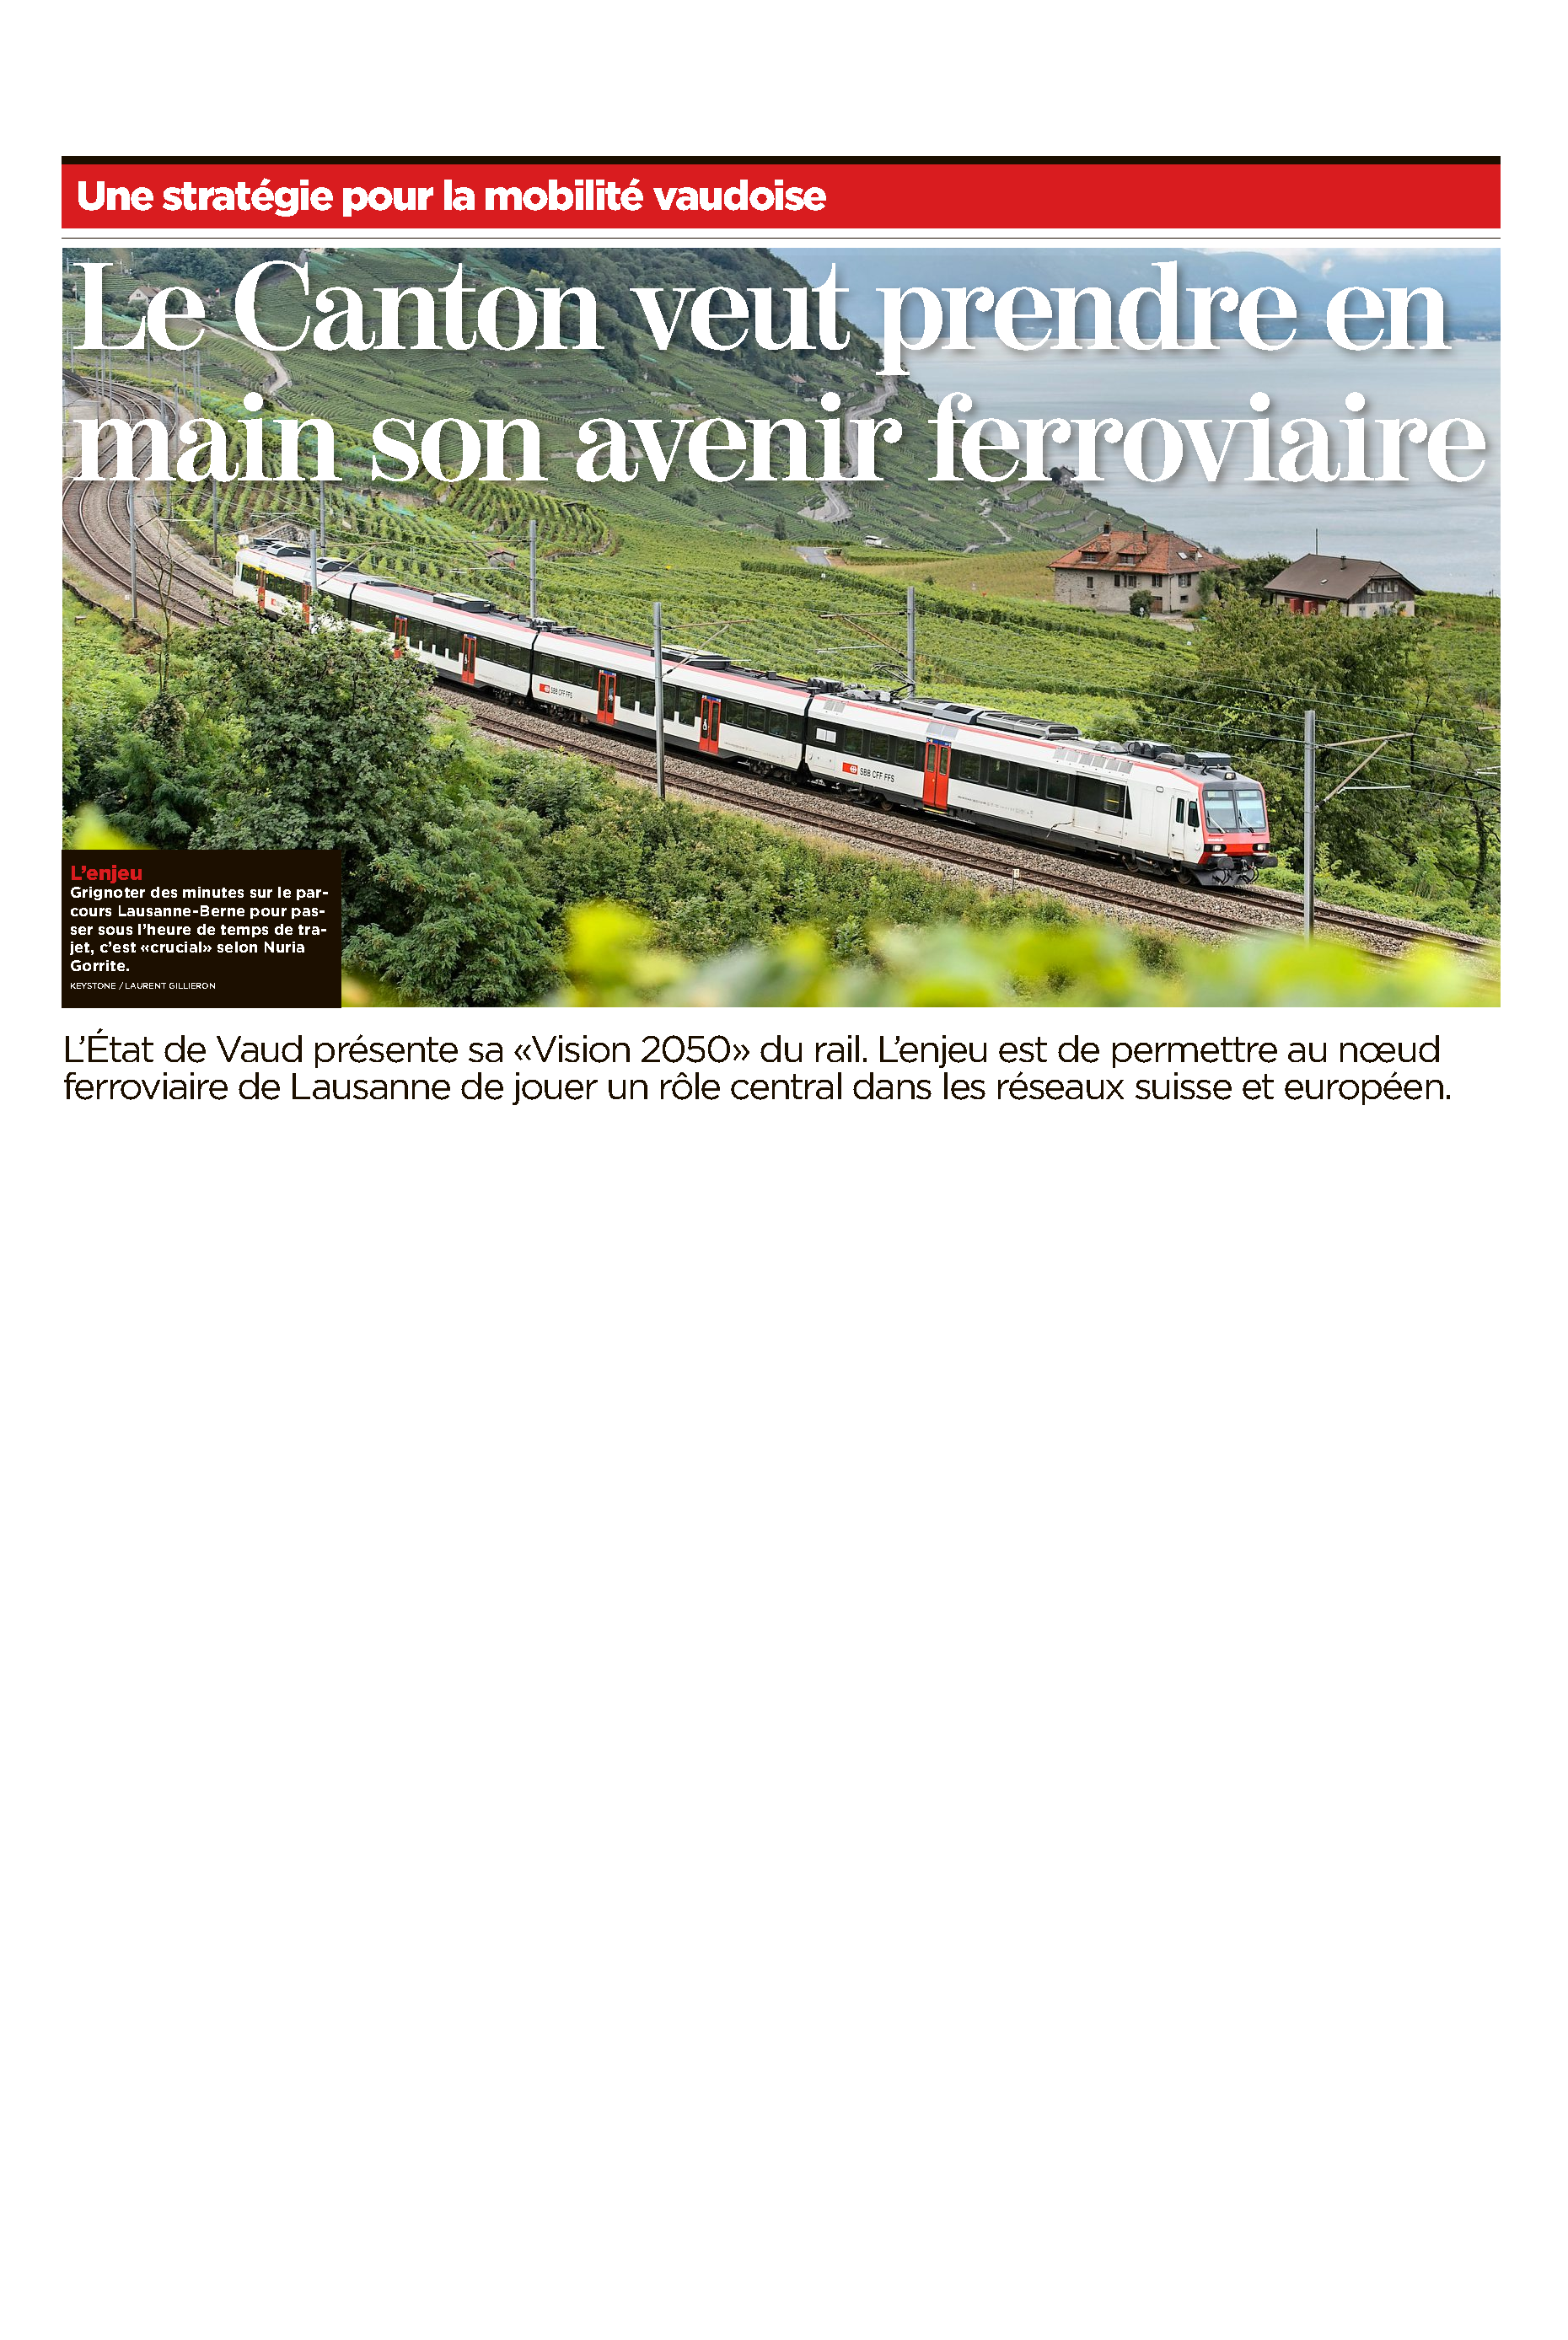
\includegraphics[scale = 0.55]{Figures/24h4.6.20bis_Conclusion.pdf}
    \caption{From 24h newspaper , “Mobility strategy for Vaud inhabitants: The Canton wants to take charge of their own railway destiny” (\cite{24hmobilite})}
    \label{fig:24h_mobility}
\end{figure}
The aim of the strategy is to develop Lausanne to be a centre pole in the Swiss and European railway networks. Canton de Vaud had also provided major guidelines to reach their goal. To name a few, here some of the possible axes from the conference paper (\cite{confvaud2050}):
\begin{enumerate}
    \itemsep0mm
    \item Create new regional services (RER Payerne-Lausanne and Vevey-Berne);
    \item Find solution for the travel time between Lausanne and Bern;
    \item Favour new  long-distance projects (Swiss and European);
    \item Optimize the freight services.
\end{enumerate}
I appreciate the audacity of the Canton to set the goals high and to try their best to challenge themselves in a very tight competition.
\par As I understand now, the launched study will be taken by professional and private rail consultants with the collaboration of the Canton. Thus, my thesis will probably not be considered in their study which gives me the opportunity to work in parallel with them, the latitude of being more creative and try out bold and innovative solutions.
\newpage
\section{The two possible axes for the Master Thesis}
With keeping the interest of the Canton in mind (\cite{vaud2050}), I am presenting here two possible axes for my master thesis which I will define during my pre-study. Each axe will be describe with a goal, a brief methodology, the needed inputs and the possible collaboration.
\subsection{Paris-Milan night train inter-city line service}
\begin{itemize}
    \itemsep0mm
    \item \textit{Goal:} Create a night inter-city line between Paris-Lausanne-Milan which is economically profitable and doesn't impact much the railways network.
    \item \textit{Methodology:} 
    \begin{enumerate}
    \itemsep 0mm
        \item Collect data on the current public transportation offers for night services.
        \item Collect railways infrastructure and railways input (i.e: SMA)
        \item Operation research with a software (i.e: Viriato)
        \item Collect OD data (i.e: LASUR lab)
        \item Market Share Forecast (i.e: Biogeme)
        \item Economic and environment impacts study
    \end{enumerate}
    \item \textit{Data:} Existing train schedule for the Paris-Lausanne-Milan line. Characteristics of the train. Market share, Origin-Destination data.
    \item \textit{Collaboration:}
    \begin{enumerate}
        \itemsep 0mm
        \item SMA (Matthias Hellwig and Matthew Holiday for the software and technical supervision on the software. \textbf{Already  in contact})
        \item Canton de Vaud (Philippe Gauderon and other involved people)
        \item Prof. Kauffman (lab LASUR)
    \end{enumerate}
\end{itemize}

\subsection{Implementation of hydrogen trains on the regional service}
\begin{itemize}
    \itemsep0mm
    \item \textit{Goal:} Study the economic feasibility, the operation feasibility and the environmental impact of implementing new hydrogen trains.
    \item \textit{Possible service lines:}
    \begin{enumerate}
        \itemsep0mm
        \item Genève - Lausanne
        \item Lausanne - Vevey
        \item Lausanne - Bern
    \end{enumerate}
    \item \textit{Methodology:}
    \begin{enumerate}
        \itemsep0mm
        \item Collect the characteristics of the Siemens hydrogen trains.
        \item Collect the characteristics of the regional service train.
        \item Collect any inputs needed about the railway infrastructure.
        \item Identifiy and design the necessary infrastructure for the hydrogen service.
        \item Operation research with a software (i.e: Viriato)
        \item Compare the two services (efficiency, reliability, cost and environment impacts)
    \end{enumerate}
    \item \textit{Data:} Regional train schedules, current train characteristics, Siemens/Alstom new hydrogen trains characteristics. Infrastructure on the service lines. Costs for regional train service. 
    \item \textit{Collaboration:} 
    \begin{enumerate}
        \itemsep 0mm
        \item Hydrogen train department (i.e : engineer department at Siemens)
        \item Canton de Vaud (Philippe Gauderon and other implied people)
        \item CFF (Prof. Hans-Jörg Stark or other)
    \end{enumerate}
\end{itemize}
\newpage
\section{Timeline}
The timeline will be divided in the major parts. The first part is the pre-study and the second one is for the thesis. I am keeping in mind that I need to put the equivalent of 90 hours of work for the pre-study to obtain the credits.

\subsection{Pre-study}
\begin{itemize}
    \item Starting: 12.12.2020 -  Ending:   21.02.2021 - Length: 2 months
    \item December: (15 hours)
    \vspace{-0.25cm}
    \begin{itemize}
        \itemsep0mm
        \item \textit{Contacting all the collaborators}
        \item \textit{Collecting the data}
        \item \textit{Learning the software}
    \end{itemize}
    \item January: (60 hours)
        \vspace{-0.25cm}
    \begin{itemize}
        \itemsep0mm
        \item \textit{Finalizing the collection of the data}
        \item \textit{Understanding the data}
        \item \textit{Implementing the data on the software}
        \item \textit{Identifying the challenges}
    \end{itemize}
    \item February: (15 hours)
        \vspace{-0.25cm}
    \begin{itemize}
        \itemsep0mm
        \item \textit{Defining the final goal and objectives of the master thesis}
        \item \textit{Presentation of the pre-study}
    \end{itemize}
\end{itemize}
\subsection{Master Thesis}
\begin{itemize}
    \item Starting: 21.02.2021 -  Ending: ??.07.2021 - Length: minimum 4 months
    \item Principals deadlines
    \begin{itemize}
        \itemsep0mm
        \item \textit{Implementation and analyze}
        \item \textit{Mid-term report and presentation}
        \item \textit{Correction and realignment based on the comments of the mid-term}
        \item \textit{Final report and presentation}
    \end{itemize}
\end{itemize}

\begin{figure}[h]
    \centering
    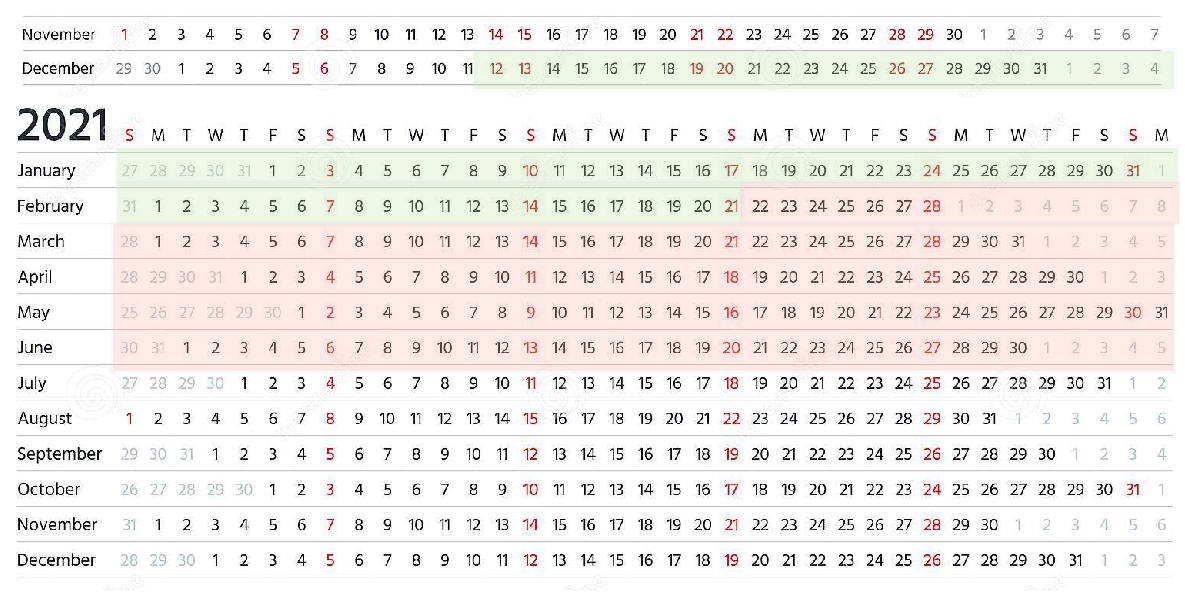
\includegraphics[scale = 0.78]{Figures/timeline.pdf}
    \caption{Proposed timeline for the pre-study (in green) and the master thesis (in red).}
    \label{fig:my_label}
\end{figure}
\newpage
\printbibliography


\end{document}

